\documentclass[letterpaper, 11pt]{article}

% set version variable
\newcommand{\versionnumber}{0.1}

% russian language
\usepackage[utf8]{inputenc}
\usepackage[T2A]{fontenc}
\usepackage[english, russian]{babel}
\usepackage{algorithmicx}
\usepackage{algpseudocode}
\usepackage{graphicx}
\usepackage{caption}
\usepackage{subcaption}
\usepackage{amsmath}
\usepackage{blkarray}
\usepackage{tikz}
\usetikzlibrary{automata,arrows,positioning,calc}


% math
\usepackage{amsmath}

\usepackage{amssymb} % some math symbols


% enumerate
\usepackage{enumerate}

% set type and margins of the page
\usepackage{geometry}  % document margins
\geometry{letterpaper, left=1.4in, right = 1.4in, top = 1.7in, bottom = 1.7in}

% color links in content
\usepackage{hyperref}
\hypersetup{
    colorlinks=true,
    linkcolor=red,
    urlcolor=blue,
    linktoc=all
}

% indent at first \par after section
\usepackage{indentfirst}

% fixed table and figures in section
\usepackage{float}

% colors
\usepackage{color}
%\usepackage[usenames,dvipsnames]{xcolor}

\newcommand{\prob}{\mathrm{P}}
\newcommand{\expe}{\mathrm{E}}
\newcommand{\var}{\mathrm{D}}
\newcommand{\tr}{\mathrm{tr}}
\newcommand{\KK}{\mathbf{K}}
\newcommand{\XX}{\mathbf{X}}
\newcommand{\MM}{\mathbf{M}}
\newcommand{\Cov}{\mathrm{Cov}}
\newcommand{\Var}{\mathrm{Var}}

\DeclareMathOperator*{\argmin}{\arg\!\min}
\DeclareMathOperator*{\argmax}{\arg\!\max}

% paragraph indent
\setlength{\parskip}{0.5em}

\title{\large{Краткий конспект}\\
\LARGE{Лекция 7. Скрытые марковские модели в биоинформатике}\\
draft version}
\date{7 марта, 2016}
\author{Д. Ищенко\thanks{МФТИ} \and Б. Коварский\footnotemark[1]
\and И. Алтухов\footnotemark[1] \and Д. Алексеев\footnotemark[1]}

\begin{document}
\maketitle
\thispagestyle{empty}
\clearpage

% let's go

На предыдущих лекциях мы научились выравнивать последовательности, сравнивать их, собирать короткие в большие, но пока что последовательность для нас это всего лишь набор символом, смысла которого мы не понимаем.
Важная задачу в вычислительной биологии - это зная биологическую последовательность, понять структурные и функциональные характеристики более высокого порядка, проаннотировать последовательность.

В случае геномной последовательности, нас интересует определение экзон-интронной структуры, поиск открытых рамок считывания, поиск 	сайтов связывания рибосом, транскрипционных факторов, геномных островов. Для последовательностей отдельных белков нас интересуют структурные особенности белка, его укладка.

Оказывается, с разной эффективностью перечисленные задачи могут быть решены при помощи скрытых марковских моделей. Более того, выравнивать последовательности также можно с использованием СММ

Для начала, вспомним, что такое марковская цепь.

\section{Марковские цепи}
\subsection{Определения}

\textit{Цепь Маркова} — последовательность дискретных случайных величин (состояний) $Q=q_0,q_1,\ldots,q_n,\ldots$, обладающая \textit{марковскми свойством}: значение случайной величины на любом шаге, зависит только от предыдущего состояния $q_{n-1}$:

$$\prob(q_{n}|q_{n-1},q_{n-2},\ldots,q_{n})=\prob(q_{n}|q_{n-1})$$

$$q_{n}\in S$$

$$S=\{s_1,\ldots,s_k,\ldots\}$$ -- конечное или счетное множество возможных состояний марковской цепи.


\textit{Марковская модель} -- вероятностная модель, описывающая последовательность событий, обладающим марковским свойством.
Таким образом, марковская модель -- минимально возможное усложнение модели независимых испытаний.

Марковская модель $\lambda=(S,A,\pi)$ однозначно задается следующим набором параметров:

\begin{enumerate}

\item множество состояний

$$S=\{s_1,\ldots,s_k,\ldots\}$$

\item матрица перехода между состояниями 

$$A=a_{ij}(n)=\prob(q_{n+1}=s_j|q_{n}=s_i)$$

Матрица перехода является стохастической матрицей: для ее строк выполняется условие $\sum\limits_{j}a_{ij}=1$

\item начальное распределение

$$\pi=(\pi_i);\quad\pi_i=\prob(q_0=s_i)$$

\end{enumerate}

Реализацией марковской модели $\lambda=(S,A,\pi)$ служит последовательность:  $Q=q_0,q_1,\ldots,q_k,\ldots$, иными словами марковская модель генерирует последовательность событий $Q$:

$$\lambda=(S,A,\pi) \rightsquigarrow Q$$

\subsection{Примеры}

Рассмотрим простейшую марковскую цепь с двумя состояниями:

$$\lambda=(S,A,\pi)$$

$$S=\{1,2\};
\quad
A=
\begin{pmatrix}
  p & (1-p) \\
  (1-q) & q \\
 \end{pmatrix};
\quad
\pi=
\begin{pmatrix}
  r \\
  1-r \\
 \end{pmatrix}
$$


Граф переходов для такой марковской цепи:

\begin{center}
\begin{tikzpicture}[->, >=stealth', auto, semithick, node distance=3cm]
\tikzstyle{every state}=[fill=white,draw=black,thick,text=black,scale=1]
\node[state]    (A)                     {$1$};
\node[state]    (B)[right of=A]   {$2$};
\path
(A) edge[loop left]     node{$p$}         (A)
    edge[bend left]     node{$1-p$}     (B)
(B) edge[loop right]     node{$q$}         (B)
    edge[bend left]     node{$1-q$}     (A);  
\end{tikzpicture}
\end{center}


Тогда вероятность наблюдать последовательность состояний (траекторию) $1\to1\to2$ при заданной марковской модели $\lambda$ будет определяться как:

\begin{gather}
\prob(Q=1,1,2|\lambda)=\prob(q_0=1)\prob(q_1=1|q_0=1)\prob(q_2=2|q_1=1)=
\pi_1 a_{11}a_{12}=rp(1-p)
\end{gather}


Если траектория неопределена, то вероятность, что мы окажемся после двух шагов в состоянии 2:

\begin{gather}
\prob(q_2=2|\lambda)=\prob(Q=1,1,2)+\prob(Q=2,1,2)+\prob(Q=1,2,2)+\prob(Q=2,2,2)=\\=
\pi_1 a_{11}a_{12}+\pi_2 a_{21}a_{12}+\pi_1 a_{12}a_{22}+\pi_2 a_{22}a_{22}
\end{gather}

Обобщим эти наблюдения для произвольной марковской цепи.

Вероятность траектории:

\begin{gather}
\prob(Q)=\prob(q_0=i_0,\ldots,q_n=i_n)=
\prod_{k=0}^n\prob(q_k=i_k|q_{k-1}=i_{k-1},\ldots,q_{0}=i_{0})=
\prod_{k=0}^n\prob(q_k=i_k|q_{k-1}=i_{k-1})=\\=
\prod_{k=0}^n\prob(q_k=i_k|q_{k-1}=i_{k-1})=\pi_{i_0}\prod_{k=1}^n a_{i_{k-1}i_{k}}
\end{gather}

Где $i_k$ - номер состояния из числа возможных 

Вероятность перехода из состояния $i_0$ в $i_n$ после $n$ шагов

$$\prob(q_n=i_n|q_0=i_0)=\sum_{i_1,\ldots,i_{n-1}}\pi_{i_0}\prod{k=1}^n a{i_{k-1}i_{k}}=(A^n){i_0,i_n}\pi_{i_0}$$

Вероятности наблюдения состояний после $n$ шагов.

$$p_n=\prob(q_n)=A^n\pi$$

То есть матрица переходных вероятностей за n шагов однородной цепи Маркова есть n-я степень матрицы переходных вероятностей за 1 шаг

Еще один пример -- случайное блуждание с отражением и с поглощением. Пускай есть частица, которая в первый момент времени имеет координату $q_0=k$. С вероятностью $p$ она движется на единицу вверх и с $1-p$ на единицу вниз. Состояния $1$ и $N$ - являются поглощающими, т.е. после их достижения уровня блуждание прекращается. Марковская модель для такого процесса при $N=5, k=3$ будет иметь вид:

$$S=\{1,2,3,4,5\};\quad
A=
\begin{pmatrix}
1 & 0 & 0 & 0 & 0\\
1-p & 0 & p & 0 & 0\\
0 & 1-p & 0 & p & 0\\
0 & 0 & 1-p & 0 & p\\
0 & 0 & 0 & 0 & 1\\
\end{pmatrix};
\quad
\pi=
\begin{pmatrix}
0\\
0\\
1\\
0\\
0\\
\end{pmatrix};
$$

Граф переходов:

\begin{center}
\begin{tikzpicture}[->, >=stealth', auto, semithick, node distance=3cm]
\tikzstyle{every state}=[fill=white,draw=black,thick,text=black,scale=1]
\node[state]    (A) {$1$};
\node[state]    (B)[right of=A]   {$2$};
\node[state]    (C)[right of=B]   {$3$};
\node[state]    (D)[right of=C]   {$4$};
\node[state]    (F)[right of=D]   {$5$};
\path
(A) edge[loop left]     node{$1$}         (A)
(B) edge[bend left]     node{$1-p$}         (A)
(C) edge[bend left]     node{$1-p$}         (B)
(D) edge[bend left]     node{$1-p$}         (C)
(B) edge[bend left]     node{$p$}         (C)
(C) edge[bend left]     node{$p$}         (D)
(D) edge[bend left]     node{$p$}         (F)
(F)    edge[loop right]     node{$1$}     (F);  
\end{tikzpicture}
\end{center}


Перейдем теперь к рассмотрению скрытой марковской модели.

\section{Скрытые марковские модели}

\subsection{Определения}

\textit{Скрытая марковская модель} — это вероятностная модель последовательности $(q_0, d_0), \ldots,(q_n,d_n),\ldots$, которая состоит из набора наблюдаемых переменных и набора скрытых переменных состояния $q_n$ . При этом значения наблюдаемой переменной $d_n$ на шаге $n$ зависит только от скрытого состояния $q_n$, которое в свою очередь зависит лишь от скрытого состояния $q_{n-1}$ на предыдущем шаге $n-1$.

Что поменялось в сравнение с обычной марковским процессом? Теперь состояния $q_n$ скрыты от наблюдателя, а судить о становится возможным по наблюдаемым $d_n$.

Скрытая марковская модель $\lambda=(S,\Sigma, A,B, \pi)$ описывается следующим набором параметров:

\begin{enumerate}


\item конечное множество состояний скрытой марковской модели:

$$S=\{s_1,\ldots,s_k\}$$

\item матрица вероятностей переходов между скрытыми состояниями

$$A=(a_{ij}); \quad a_{ij}=\prob(s_j|s_i)$$

\item алфавит, множество наблюдаемых скрытой марковской модели

$$\Sigma=\{x_1,\ldots,x_m\}$$

\item матрица вероятностей эмиссий, т.е. вероятностей получить наблюдаемую $x_k$, находясь в состоянии $s_j$

$$B=(b_{jk});\quad b_{ik}=p(x_k|s_j)$$

\item начальное распределение

$$\pi=(\pi_i);\quad\pi_i=\prob(q_0=s_i)$$

\end{enumerate}


Реализацией СММ является набор из двух последовательностей:

\begin{itemize}

\item наблюдения (данные):
	$$D=(d_0,d_1,\ldots,d_n)$$
	
\item скрытые состояния (траектория цепи)

$$Q=(q_0,q_1,\ldots,q_n)$$

\end{itemize}

$$\lambda=(S,\Sigma, A,B)\rightsquigarrow (D,Q)$$

\subsection{Задача о подмене монеты}

Для иллюстрации рассмотрим задачу о подмене монеты. Допустим некто играет с вами в орлянку, подбрасывает монету, сообщая вам лишь результат -- орел или решка, самой монеты вы не видите. При этом ваш противник не слишком честен и изредка он делает подмену правильной монеты на фальшивую у которой одна из сторон выпадает чаще (скажем, решка в 75\% случаев) и наоборот. Можете ли вы глядя на результат -- последовательность орлов и решек, определить в какой момент наиболее вероятно были произведены подмены?

Опишем  процесс в терминах СММ.

Имеется два скрытых состояния - фальшивая монета ($F$, \textit{false}) либо нет ($N$, \textit{normal}) и две наблюдаемых - орел ($H$, \textit{heads}) либо решка ($T$, \textit{tails})
$$S=\{F,N\};\quad \Sigma=\{H,T\}$$

Вероятности переходов, допустим:

$$A=
\begin{blockarray}{ccc}
F & N \\
\begin{block}{(cc)c}
0.9 & 0.1 & F \\
0.1 & 0.9 & N \\
\end{block}
\end{blockarray}
$$

Вероятности наблюдаемых:

$$B=
\begin{blockarray}{ccc}
H & T \\
\begin{block}{(cc)c}
0.25 & 0.75 & F \\
0.5 & 0.5 & N \\
\end{block}
\end{blockarray}
$$

Начальное распределение:

$$\pi=
\begin{pmatrix}
0 \\
1 \\
\end{pmatrix}
$$

  
Последовательность наблюдений:
$D=(H,H,T,T,H,T,T,T,T,H)$

Последовательность скрытых состояний:
$Q=(N,N,N,N,N,F,F,F,F,N)$

Данную СММ можно изобразить в виде графа переходов:

\begin{center}
\begin{tikzpicture}[->, >=stealth', auto, semithick, node distance=3cm]
\tikzstyle{every state}=[fill=white,draw=black,thick,text=black,scale=1]
\node[state]    (N) {$N$};
\node[state]    (F)[right of=N]   {$F$};
\node[state]    (H)[below of=N,draw=red]   {$H$};
\node[state]    (T)[below of=F,draw=red]   {$T$};
\path
(N) edge[loop left]     node{$0.9$}         (N)
(F) edge[loop right]     node{$0.9$}         (F)
(F) edge[bend left]     node{$0.1$}         (N)
(N) edge[bend left]     node{$0.1$}         (F)
(N) edge     node{$0.5$}         (H)
(N) edge     node{$0.5$}         (T)
(F) edge     node{$0.25$}         (H)
(F) edge     node{$0.75$}         (T);
\node[left=2cm] (N){\textit{Скрытые состояния:}};
\node[below left=3.5cm] (N){\textit{Наблюдаемые:}};
\end{tikzpicture}
\end{center}



Последовательность скрытых состояний может быть изображена как траектория на направленном ациклическом графе всевозможных траекторий переходов между скрытыми состояниями:

\begin{center}
\begin{tikzpicture}[->, >=stealth', auto, semithick, node distance=3cm]
\tikzstyle{every state}=[fill=white,draw=black,thick,text=black,scale=0.5]
\node[state]    (N1) {$N$};
\node[state]    (F1)[below of=N1]   {$N$};

\node[state]    (N2)[right of=N1]  {$N$};
\node[state]    (F2)[right of=F1]   {$F$};

\node[state]    (N3)[right of=N2]  {$N$};
\node[state]    (F3)[right of=F2]   {$F$};

\node[state]    (N4)[right of=N3]  {$N$};
\node[state]    (F4)[right of=F3]   {$F$};

\node[state]    (N5)[right of=N4]  {$N$};
\node[state]    (F5)[right of=F4]   {$F$};

\node[state]    (N6)[right of=N5]  {$N$};
\node[state]    (F6)[right of=F5]   {$F$};

\node[state]    (N7)[right of=N6]   {$N$};
\node[state]    (F7)[right of=F6]  {$F$};

\node[state]    (N8)[right of=N7]   {$N$};
\node[state]    (F8)[right of=F7]  {$F$};

\node[state]    (N9)[right of=N8]   {$N$};
\node[state]    (F9)[right of=F8]  {$F$};

\node[state]    (N10)[right of=N9]   {$N$};
\node[state]    (F10)[right of=F9]  {$F$};

\path
(N1) edge     node{}         (F2)
(N1) edge[draw=red]     node{}         (N2)
(F1) edge     node{}         (F2)
(F1) edge     node{}         (N2)
(N2) edge     node{}         (F3)
(N2) edge[draw=red]     node{}         (N3)
(F2) edge     node{}         (F3)
(F2) edge     node{}         (N3)
(N3) edge     node{}         (F4)
(N3) edge[draw=red]     node{}         (N4)
(F3) edge     node{}         (F4)
(F3) edge     node{}         (N4)
(N4) edge     node{}         (F5)
(N4) edge[draw=red]     node{}         (N5)
(F4) edge     node{}         (F5)
(F4) edge     node{}         (N5)
(N5) edge[draw=red]     node{}         (F6)
(N5) edge     node{}         (N6)
(F5) edge     node{}         (F6)
(F5) edge     node{}         (N6)
(N6) edge     node{}         (F7)
(N6) edge     node{}         (N7)
(F6) edge[draw=red]     node{}         (F7)
(F6) edge     node{}         (N7)
(N7) edge     node{}         (F8)
(N7) edge     node{}         (N8)
(F7) edge[draw=red]     node{}         (F8)
(F7) edge     node{}         (N8)
(N8) edge     node{}         (F9)
(N8) edge     node{}         (N9)
(F8) edge[draw=red]     node{}         (F9)
(F8) edge     node{}         (N9)
(N9) edge     node{}         (F10)
(N9) edge     node{}         (N10)
(F9) edge     node{}         (F10)
(F9) edge[draw=red]     node{}         (N10);
\end{tikzpicture}
\end{center}


Для определения моментов подмены монеты мы должным подобрать среди всех возможных последовательностей скрытых состояний (траекторий) такую, при которых вероятность наблюдать последовательность $D$ максимальна, т.е. мы должны решить следующую задачу:

$$Q^*=\argmax_Q P(D,Q|\lambda)$$

\subsection{Анализ биологических последовательностей при помощи СММ}

Какое отношение орлянка имеет к анализу биологических последовательностей? Биологическую последовательность можно воспринимать как последовательность наблюдений (аминокислот и нуклеотидов), за которыми скрываются неизвестные биологические свойства (скрытые состояния). Рассмотрим два примера. 

\subsubsection{Поиск геномных островов}

Первый пример -- поиск геномных островов. Геномные острова -- кластеры генов в геномах прокариот, приобретаемые посредством горизонтального переноса. Когда в 1990х исследовали геномы кишечной палочки оказалось, что патогенные и непатогенные штаммы в сущности отличаются наличием или отсутствием определенных кластеров генов, расположенными в нестабильных регионах хромосом, из чего следует что кластеры скорее всего были приобретены горизонтально. Подобные кластеры получили название острова патогенности. В островах патогенности могут находятся разнообразные токсины (гемолизин кишечной палочки, пестицин чумной палочки), адгезины, позволяющие бактерии прикрепляться, суперантигены (вызывающие массовую активацию неспецифическую активацию T-лимфоцитов и как следствие инфекционно-токсический шок). Но островками патогенности все не ограничилось. Затем были обнаружены иные острова: метаболические острова, симбиотические острова, острова резистентности.


\begin{figure}
\centering
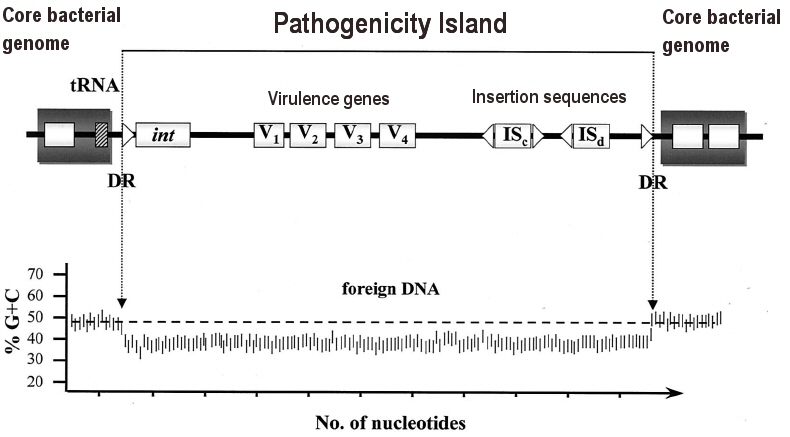
\includegraphics[height=7cm]{images/island.png}
\caption{Упрощенная схема строения острова патогенности. $IS$-insertion sequence, $int$-интеграза, $V_1,\ldots,V_4$ - гены вирулентности, $DR$ -прямые повторы. Иллюстрация из \textit{Herbert Schmidt and Michael Hensel, Clinical Microbiology Reviews, January 2004, Vol. 17, p. 14-56.}}
\label{fig:island}
\end{figure}



Геномные острова имеют вполне узнаваемую структуру. Их длина несколько десятков тысяч нуклеотидов, они часто фланкированы прямыми повторами, внутри островов присутствуют гены обеспечивающие мобильность (интегразы или транспозазы) и специфичные гены (токсины, гены резистентности). Для нас же важно то, что $k$-мерный спектр (частоты встречаемости нуклеотидных подстрок длины $k$) в островах,  отличается от геномного. В частности у геномных островов иной GC-состав


В терминах СММ в данной задачи наблюдаемые - нуклеотиды, взятые из алфавита $\Sigma=\{A,T,G,C\}$, а скрытые состояния, находится ли данный нуклеотид внтури острова или нет $S=\{I,N\}$. Геномные острова и части генома не относящиеся к ним состоят из целого блока нуклеотидов, а потому вероятности переходов между скрытыми состояниями малы, это позволяет эффективно применять СММ.

Допустим, GC-состав острова $\sim 40\%$, генома $\sim 60\%$, тогда:

$$\prob(G|I)=\prob(C|I)=0.2;\quad \prob(A|I)=\prob(T|I)=0.3$$
$$\prob(G|N)=\prob(C|N)=0.3;\quad \prob(A|N)=\prob(T|N)=0.2$$

Граф переходов будет выглядеть как:

\begin{center}
\begin{tikzpicture}[->, >=stealth', auto, semithick, node distance=3cm]
\tikzstyle{every state}=[fill=white,draw=black,thick,text=black,scale=1]
\node[state]    (I) {$I$};
\node[state]    (N)[right of=I]   {$N$};
\node[state]    (T)[below of=I,draw=red]   {$T$};
\node[state]    (A)[left of=T,draw=red]   {$A$};
\node[state]    (G)[below of=N,draw=red]   {$G$};
\node[state]    (C)[right of=G,draw=red]   {$C$};

\path
(I) edge[loop left]     node{$p$}         (I)
(N) edge[loop right]     node{$p$}         (N)
(I) edge[bend left]     node{$1-p$}         (N)
(N) edge[bend left]     node{$1-p$}         (I)
(I) edge[bend right]     node{$0.3$}         (A)
(N) edge     node{$0.2$}         (A)
(I) edge[bend right]     node{$0.3$}         (T)
(N) edge     node{$0.2$}         (T)
(I) edge     node{$0.2$}         (G)
(N) edge[bend left]     node{$0.3$}         (G)
(I) edge     node{$0.2$}         (C)
(N) edge[bend left]     node{$0.3$}         (C);
\node[left=2cm] (N){\textit{Скрытые состояния:}};
\end{tikzpicture}
\end{center}

Для определения границ острова будет решаться та же самая задача, что и в примере с фальшивой монетой: $$Q^*=\argmax_Q P(D,Q|\lambda)$$

%Построим СММ, при помощи которой можно было бы решить задачу поиска островов.
%Наблюдаемыми состояниями у нас является последовательность нуклеотидов
%
%Алфавит?
%$D=(A,G,T,T,T,A,G,C,C,G,C,T,C)$
%
%Состояния - находится ли данный нуклеотид в геномном острове или нет.
%
%$Q=(N,N,N,N,I,I,I,I,I,I,I,I,I)$



%Сравним задачу про монету и поиск островов, 
%
%Возникает проблема откуда взять вероятности $A,B,\pi$? Ответ - из данных нужно обучить СММ. Так что СММ - метод машинного обучения.К вопросу как обучать СММ мы еще вернемся.

\subsubsection{Определение структуры трансмембранных белков}

Второй пример -- это определение доменов трансмембранных белков. Трансмембранные белки насквозь пронизывают липидный бислой, при этом часть их находится внутри мембраны, а часть - снаружи клетки, часть внутри цитоплазмы. Внутри мембраны чаще располагаются гидрофобные белки, снаружи - гидрофильные, как видно на примере бактериородопсина (рис. ~\ref{fig:rhodopsin}).

\begin{figure}
        \centering
        \begin{subfigure}[b]{0.39\textwidth}
                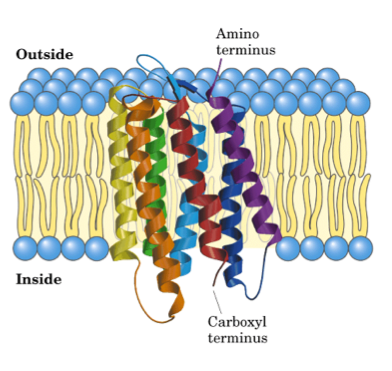
\includegraphics[width=\textwidth]{images/rhodopsin.png}
                \caption{}
                \label{fig:rhod1}
        \end{subfigure}
        ~ %add desired spacing between images, e. g. ~, \quad, \qquad, \hfill etc.
          %(or a blank line to force the subfigure onto a new line)
        \begin{subfigure}[b]{0.55\textwidth}
                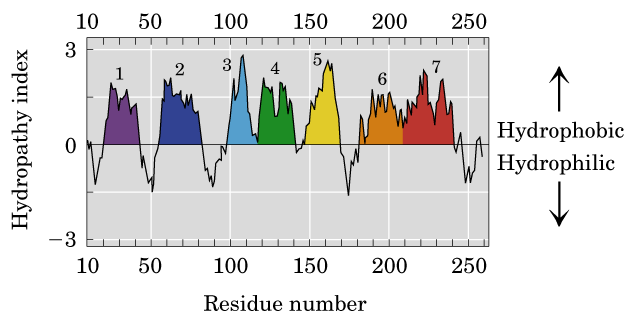
\includegraphics[width=\textwidth]{images/rhodopsin2.png}
                \caption{}
                \label{fig:rhod2}
        \end{subfigure} 
        \caption{(а) структура бактериородопсина; (b) индекс гидропатии для разных аминокислотных остатков бактериородопсина. Иллюстрация из \textit{Lehninger Principles of Biochemistry, 3rd ed., 2000}}\label{fig:rhodopsin}
\end{figure}



В простейшей СММ для определения внутримембранных регионов двадцатисимвольный аминокислотный алфавит можно редуцировать до двухбуквенного: $\Sigma=\{H(hydrophobic), L(hydrophylic)\}$ и рассматривать три скрытых состояния: $S=\{E(extracellular), M(membrane), C(cytoplasmic)\}$

Граф переходов:

\begin{center}
\begin{tikzpicture}[->, >=stealth', auto, semithick, node distance=3cm]
\tikzstyle{every state}=[fill=white,draw=black,thick,text=black,scale=1]
\node[state]    (E) {$E$};
\node[state]    (M)[right of=E]   {$M$};
\node[state]    (C)[right of=M]   {$C$};

\node[state]    (H)[below of=E,draw=red]   {$H$};
\node[state]    (L)[below of=C,draw=red]   {$L$};

\path
(E) edge[loop left]     node{}         (E)
(C) edge[loop right]     node{}         (C)
(M) edge[loop above]     node{}         (M)
(E) edge[bend left]     node{}         (M)
(M) edge[bend left]     node{}         (C)
(M) edge[bend left]     node{}         (E)
(C) edge[bend left]     node{}         (M)
(C) edge     node{}         (L)
(C) edge     node{}         (H)
(M) edge     node{}         (L)
(M) edge     node{}         (H)
(E) edge     node{}         (L)
(E) edge     node{}         (H);
\end{tikzpicture}
\end{center}

Как видно, особенность данной СММ, что вероятности переходов $p(E|C)=p(C|E)=0$, так как мы не можем оказаться внутри клетки, не пройдя через мембрану.

\subsection{Алгоритмические задачи, связанные с СММ}

С СММ связаны три основные задачи

\begin{enumerate}

\item Уже упомянутая \textit{задача распознавания}: определение наиболее вероятной последовательности скрытых состояний при заданных параметрах СММ $\lambda$ и последовательности наблюдаемых:

$$Q^*=\argmax_Q \prob(D,Q|\lambda)$$

Задача решается при помощи \textit{алгоритма Витерби}.

\item \textit{Определение правдоподобия модели}: определение вероятности получить последовательность наблюдаемых $Q$ при заданных параметрах СММ $\lambda$:

$$L=\prob(D|\lambda)$$

Оценка правдоподобия модели позволяет из конечного набора конкурирующих моделей $\lambda_1,\lambda_2,\ldots,\lambda_n$ выбирать из них наиболее правдоподбную:

$$\lambda^*=\argmax_{\lambda_1,\lambda_2,\ldots,\lambda_n}\prob(D|\lambda_i)$$

Задача решается при помощи \textit{алгоритма просмотра вперед}.

\item \textit{Обучение СММ без учителя}: подобрать набор параметров СММ $\lambda$ при котором вероятность наблюдать последовательность $Q$ максимальна:

$$\lambda^*=\argmax_{\lambda}\prob(D|\lambda)$$

В отличие от предыдущей задачи у нас нет конечного набора заданных СММ, вместо этого требуется найти СММ среди всевозможных значений параметров. Задача решается при помощи \textit{алгоритма Баума-Велша}.


\end{enumerate}

\section{Алгоритмы}

Последовательность скрытых состояний - образует путь в направленном ациклическом графе переходов между скрытыми состояниями. Задачи на направленных ациклических графах как мы знаем хорошо решаются при помощи динамического программирования.

\subsection{Задача распознавания. Алгоритм Витерби}

$$Q^*=\argmax_Q \prob(D,Q|\lambda)$$

Для начала допустим, что последовательности скрытых состояний $Q$ заданы, как и наблюдаемые $D$:

$$D=(d_0,d_1,d_2,\ldots,d_n)$$
$$Q=(q_0,q_1,q_2,\ldots,q_n)$$

Тогда:
$$\prob(D,Q|\lambda)=\prob(D|Q,\lambda)\prob(Q,\lambda)$$

$$\prob(D|Q,\lambda)=\prob(d_0|q_0)\prob(d_1|q_1)\ldots\prob(d_n|q_n)=\prod_{i=0}^n\prob(d_i|q_i)$$

$$\prob(Q|\lambda)=\prob(q_0)\prob(q_1|q_0)\ldots\prob(q_n|q_{n-1})=\prob(q_0)\prod_{i=1}^n\prob(q_i|q_{i-1})$$

$$\prob(D,Q|\lambda)=\prob(q_0)\prob(d_0|q_0)\prod_{i=1}^n\prob(d_i|q_i)\prob(q_i|q_{i-1})$$

Вместо произведения вероятностей можно рассматривать сумму логарифмов, что вычислительно удобнее :

$$\log\prob(D,Q|\lambda)=\log\prob(q_0)+\log\prob(d_0|q_0) + \sum_{i=1}^n\log(\prob(d_i|q_i)\prob(q_i|q_{i-1}))$$

Проблема в том, что в действительности мы не знаем последовательность $Q$, перебирать же всевозможные траектории и находить $\prob(D,Q|\lambda)$ вычислительно неэффективно.

Чтобы не перебирать все траектории по аналогии с задачей поиска оптимального выравнивания мы можем запоминать на каждом шаге СММ для каждого скрытого состояния какая оптимальная траектория приводит в это состояние. Для этого в алгоритме Витерби определяется следующая вспомогательная величина:

\begin{gather}
v_{l,i}=\max_{q_0,\ldots,q_{l-1}}\prob(d_0,d_1,\ldots,d_l,q_0,q_1,\ldots,q_l=s_i|\lambda)=\\=
\prob(d_{l}|q_{l}=s_i,\lambda) \max_{q_0,\ldots,q_{l-1}}\prob(d_0,d_1,\ldots,d_{l-1},q_0,q_1,\ldots,q_l=s_i|\lambda)
\end{gather}

Она имеет следующий смысл: это максимальная вероятность наблюдать последовательность $d_0,d_1,\ldots,d_l$ среди всевозможных произвольных траекторий длины $l$: $q_0,q_1,\ldots,q$, заканчивающихся в состоянии $s_i$.
$v_{l,i}$

По индукции можно получить формулу для пересчета $v_{l,i}$ на каждом шаге на основе значений на предыдущем шаге:

$$v_{l+1,j}=\prob(d_{l+1}|q_{l+1}=s_j,\lambda)*\max_i(v_{l,i}\prob(q_{l+1}=s_j|q_{l}=s_i,\lambda))$$

Это приводит нас к следующей процедуре для определения наиболее вероятной последовательности скрытых состояний $Q^*$

\begin{algorithmic}[2]
\Procedure{Viterbi}{$A,B,\pi,D$}
\State $V\gets [\quad]$\Comment{Массив для хранения вероятностей наиболее вероятных путей}
\State $T\gets [\quad]$\Comment{Массив для хранения направлений перехода}
\For{$s\gets 0, k-1$}
\State $V[0,s]\gets \pi[s]*B[D[0],s]$
\EndFor

\For{$n\gets 1, N$}
\For{$t\gets 0, k-1$}
\State $V[n,t]\gets \max_s(V[n-1,s]*A[s,t])*B[D[n],t]$
\State $T[n,t]\gets \argmax_s(V[n-1,s]*A[s,t])$
\EndFor
\EndFor

\State $S_{fin}\gets \argmax_s(V[N,s])$

\Return $T, S_{fin}$
\EndProcedure

\end{algorithmic}

Процедура восстановления пути аналогична задачи выравнивания:

\begin{algorithmic}[2]
\Procedure{RestoreHiddenPath}{$T, S_{fin}$}

\ldots

\Return $Q$
\EndProcedure
\end{algorithmic}

\subsection{Алгоритм просмотра вперед}

Задача определения правдоподобия модели решается при помощи алгоритма просмотра вперед.

В задаче необходимо определить вероятность $\prob(D|\lambda)$. Для этого нужно просуммировать по всем возможным траекториям $Q$ уже знакомые по прошлой задаче вероятности $\prob(D,Q|\lambda)$.

\begin{gather}
\prob(D|\lambda)=\sum_{Q} \prob(D,Q|\lambda)=\sum_{Q}\prob(D|Q,\lambda)\prob(Q|\lambda)
\end{gather}

Сам алгоритм схож с алгоритмом Витерби, но вместо $v_{l,i}$ для эффективного пересчета вводится величина $\alpha_{l,i}$:

$$\alpha_{l,i}=\prob(d_0,d_1,\ldots,d_l,q_l=s_i|\lambda)=\sum_{q_0,q_1,\ldots,q_{l-1}}\prob(d_0,d_1,\ldots,d_l,q_0,q_1,\ldots,q_l=s_i|\lambda)$$

$\alpha_{l,i}$ - суммарная по всевозможным траекториям длины $l$: $q_0,q_1,\ldots,q$, заканчивающихся в состоянии $s_i$ вероятность наблюдать последовательность $d_0,d_1,\ldots,d_l$.

Для пересчета используется формула:

$$\alpha_{l+1,j}=\prob(d_{l+1}|q_{l+1}=s_j,\lambda)*\sum_i(\alpha_{l,i}\prob(q_{l+1}=s_j|q_{l}=s_i,\lambda))$$

Правдоподобие модели: $\prob(D|\lambda)=\max_i(\alpha_{n,i})$ 

%$$s_{ij}=
%\max
%\begin{pmatrix}
%	s_{i-1,j}-1, \\
%	s_{i,j-1}-1, \\
%	s_{i-1,j-1}-[v_i\ne w_j]+[v_i = w_j]
%\end{pmatrix}$$



\section{Ссылки}
\begingroup
\renewcommand{\section}[2]{}%
\begin{thebibliography}{7}
\bibitem{Frank}
\href{http://www.ece.ucsb.edu/Faculty/Rabiner/ece259/Reprints/tutorial%20on%20hmm%20and%20applications.pdf}{A tutorial on Hidden Markov Models and selected applications in speech recognition - Proceedings of the IEEE, 1989}
\bibitem{Frank}
\href{http://logic.pdmi.ras.ru/~sergey/teaching/asr/notes-09-hmm.pdf}{Лекции Сергея Николенко в Академическом университете}
\bibitem{Frank}
\href{http://www.machinelearning.ru/wiki/images/8/83/GM12_3.pdf}{Лекции Дмитрия Ветрова на ВМК}
\bibitem{Frank}
Jones N., Pevzner P. An Introduction to Bioinformatics Algorithms – MIT Press, 2004.
\end{thebibliography}


\end{document} 